\documentclass{article}
\usepackage[utf8]{inputenc}
\usepackage{amsmath}
\usepackage{amsfonts}
\usepackage{mathrsfs}
\usepackage{graphicx}
\usepackage{subcaption}
\usepackage{hyperref}
\usepackage[top=20truemm,bottom=20truemm,left=20truemm,right=20truemm]{geometry}

\title{Project Proposal}
\author{Kansuke Ikehara (Kansuke.Ikehara@colorado.edu)}

\begin{document}
\maketitle
Stochastic Block Model (SBM) is a generative model used for generating random networks with some structures, including community structure, core-periphery structure, etc. Often times, people have focused on inference using the model in order to find some sort of structure in real world data by fitting a SBM model to the data \cite{SBM, SBM_CorePeriphery}. In this model, each node (vertex) is assigned to one of communities. Edges are placed between nodes with the probability $p$ which depends on the nodes' membership to the communities. For example, nodes in the same group, say $c_{1}$ could more likely be connected than those which both are in different groups, $c_{i}$ and $c_{j}$, where $i,j \neq 1$. One of the advantages of SBM is that we could control the structure of a network with a handful parameters. 

Recent years have witnessed lines of research focusing on dynamic aspects of network modeling. Although Stochastic Block Model is a static network model, it can easily be extended to a dynamical (temporal) model \cite{DynamicalSBM,SBTM}. The studies on dynamical SBM are mainly dedicated to developing inference methods: given a series of network snapshots in which each node belongs to a group, they try to infer the node's membership and/or removal or addition of edges in the future time steps with the model. In this study, we do the opposite: we generate a triplet of parameters which governs the structure of a SBM according to a chaotic equation, generate a network with these parameters and repeat the process in the next time step. This dynamic network generation mechanism with an underlying chaos could be a testbed for those inference methods. 

A chaotic attractor we use for parameter generation is R$\ddot{\text{o}}$ssler attractor, whose trajectory is generated by the RK4 solver we have developed for homework sets. Three coordinates of R$\ddot{\text{o}}$ssler system, x,y and z are converted into three parameter $\gamma$, $p_{in}$ and $p_{out}$ respectively. $\gamma$ governs the ratio of size of two communities in our model, $p_{in}$ and $p_{out}$ are the edge probabilities for within- and between-communities. Fig.\ref{1} shows a sequence of snapshots of the generated SBM networks every 3 steps. As time proceeds the generated networks become sparser and eventually becomes dense again with a vivid community structure.

Since visualization of networks provides us only qualitative information, we will have to use network static features in order to see how two sequences of networks with different initial conditions on R$\ddot{\text{o}}$ssler attractor evolve differently over time. Candidate network statistics are: clustering coefficient, network modularity and mean geodesic distance. Plotting changes of these network statistics over time depicts how the network structure evolves over time.

\begin{figure}[h]
  \centering
  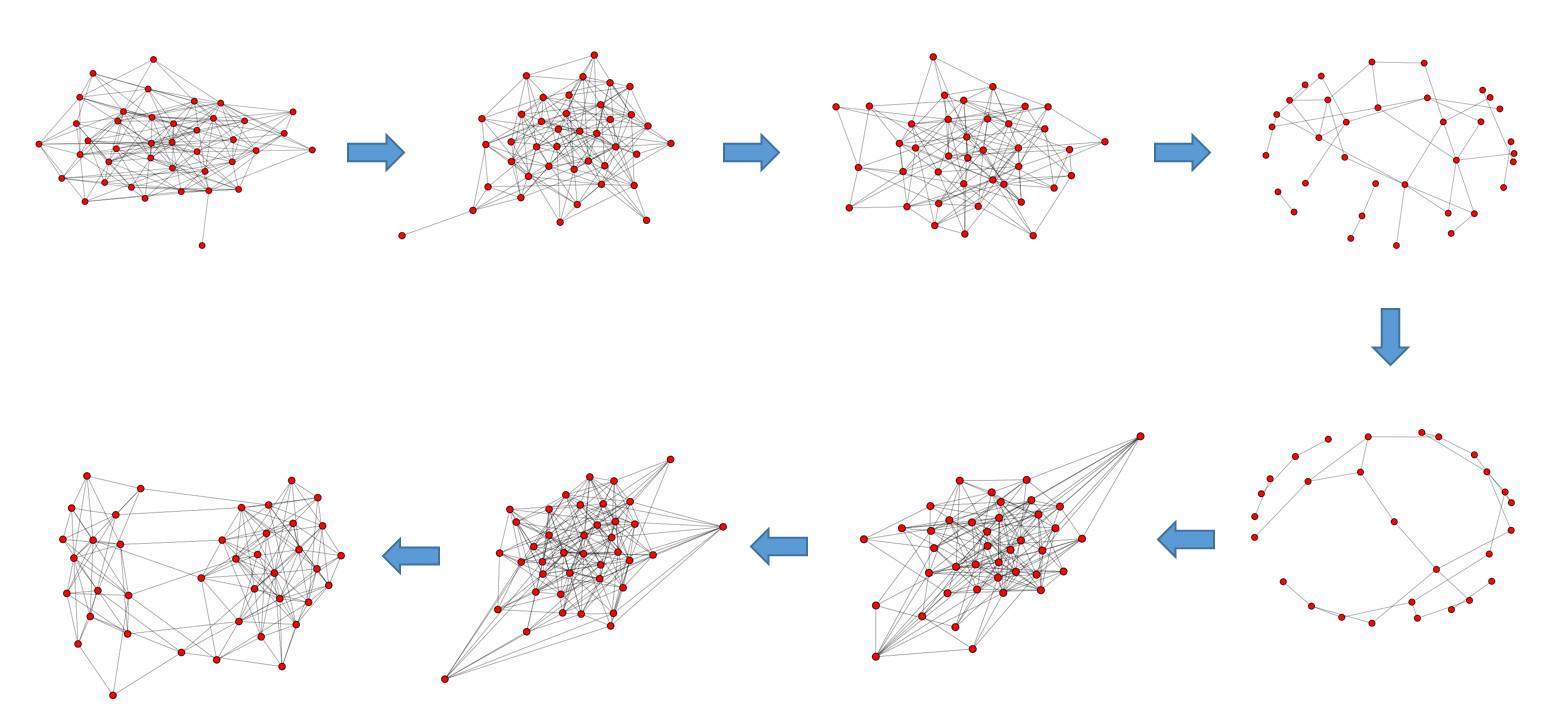
\includegraphics[height=2.5in]{figs/evolution.png}
  \caption{Snapshots of generated networks. It starts with $t = 0$ and shows networks every 3 steps.}
  \label{1}
\end{figure}

\bibliographystyle{ieeetr}
\bibliography{reference} 
\end{document}












